\section{弯曲液面的特性}


\begin{frame}
    \frametitle{弯曲液面的附加压力}

    表面弯曲的液体与平面液体有所不同，因为表面张力的存在，总是力图收缩液体表面积，这导致弯曲液体界面上承受着一定的附加压力。
    \begin{figure}[htpb]
        \centering
        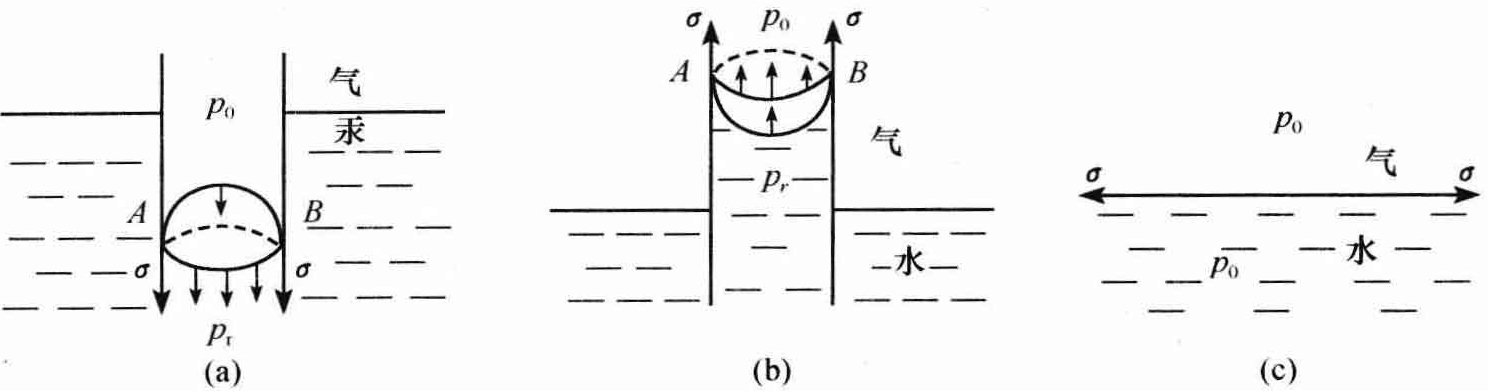
\includegraphics[width=\linewidth]{figures/fig8.2.png}
    \end{figure}
    \begin{itemize}
        \item 凸面，表面张力方向与周界垂直，指向汞的内部。 $\Delta p = p_r - p_0 > 0$
        \item 凹面，在交界线AB上作用的表面张力方向指向气相。$\Delta p < 0$
    \end{itemize}

\end{frame}


\begin{frame}
    \frametitle{拉普拉斯公式}

        \begin{minipage}{0.78\linewidth}
            若给毛细管上方活塞稍稍加压，可逆地使液滴半径增大d$r$，
            \[
                \delta W' = \dif G
            \]
            \[
                \Delta p \dif V = \sigma \dif A
            \]
            \[
                \Delta p \times 4 \pi r^2 \dif r = \sigma \times 8 \pi r \dif r
            \]
            \[
                \magenta{\Delta p = \frac{2\sigma}{r}}
            \]            
        \end{minipage}\hfill
        \begin{minipage}{0.18\linewidth}
            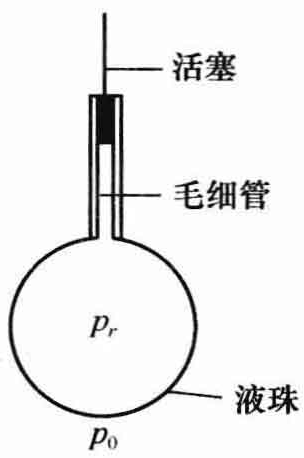
\includegraphics[width=\linewidth]{figures/fig8.3.png}
        \end{minipage}

        \begin{itemize}
            \item 附加压力与曲率半径有关。液滴越小，则所受到的附加压力值$\Delta p$越大。
            \item 弯曲液面为凸面，曲率半径为正，$r>0$，$\Delta p >0$。凹面反之。
            \item 空气中的肥皂泡，泡内气体压力大于泡外压力，因液膜有内外两个表面，其半径也近似相同，压力差值$\Delta p = \frac{4\sigma}{r}$。
            \item 平面液体，曲率半径$r \to \infty$，$\Delta p =0$。
        \end{itemize}

\end{frame}


\begin{frame}[t]
    \frametitle{}
    \begin{example}
        玻璃管两端各有一大一小肥皂泡，若将中间的旋塞打开使两气泡相通，将发生什么变化？为什么？
        \begin{figure}[htpb]
            \centering
            
\includegraphics[width=.4\linewidth]{肥皂泡}
        \end{figure}
    \end{example}
\end{frame}


\begin{frame}
    \frametitle{拉普拉斯公式的应用$-$毛细管法测液体表面张力}

    当把毛细管插入水中时，管中水柱呈凹形曲面，并上升至一定高度$h$。
    \[
        \Delta p = \frac{2\sigma}{r} = \Delta \rho gh
    \]
    $\Delta \rho = \rho_\text{液} - \rho_\text{气}$，一般$\rho_\text{液} \gg \rho_\text{气}$，故
    \[
        h = \frac{2\sigma}{\rho gr} = \frac{2\sigma}{\rho gR}
    \]
        \begin{minipage}{0.78\linewidth}
            因水能润湿玻璃毛细管，故弯曲面的曲率半径$r$近似于毛细管半径$R$。测定了毛细上升高度$h$和管径$R$，可求出液体的表面张力值。

            更一般的情况是管内液面只是球面的一部分，$R = r \cos \theta$
            \[
                h = \frac{2\sigma \cos \theta}{\rho gR}
            \]
        \end{minipage}\hfill
        \begin{minipage}{0.18\linewidth}
            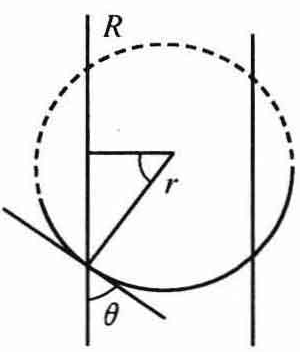
\includegraphics[width=\linewidth]{figures/fig8.5.png}
        \end{minipage}
    
\end{frame}


\begin{frame}
    \frametitle{弯曲液面的蒸气压}

    设在一定温度时，1 mol平面液体与其蒸气达到平衡，$\mu _\mathrm{l} = \mu _\mathrm{g}$。若液面曲率发生变化，如将平面液体分散成半径为$r$的小液滴，因附加压力的存在，液体所受压力由$p_0$变成$p_r$，相应地其饱和蒸气压发生改变，由$p_0^*$变为$p_r^*$，并重新建立平衡，$\dif \mu _\mathrm{l} = \dif \mu _\mathrm{g}$。当温度一定时，对于纯液体$\dif \mu _\mathrm{l} = V_\mathrm{m,l} \dif p$。假定蒸汽为理想气体，$\dif \mu _\mathrm{g} = V_\mathrm{m,g} \dif p^* = \frac{RT}{p^*}\dif p^* = RT \dif \ln p^*$，故
    \[
        V_\mathrm{m,l} \dif p = RT \dif \ln p^* 
    \]
    积分
    \[
        \int_{p_{0}}^{p_{r}} V_{\mathrm{m}, 1} \mathrm{~d} p=\int_{p_{0}^{*}}^{p_{r}^{*}} R T \mathrm{~d} \ln p^{*}
    \]
    \[
        V_{\mathrm{m}, l}(p_{r}-p_{0})=R T \ln \frac{p_{r}^{*}}{p_{0}^{*}}
    \]

\end{frame}


\begin{frame}
    \frametitle{弯曲液面的蒸气压}

    $p_{r} - p_{0} = \frac{2\sigma}{r}$，液体的摩尔体积$V_\mathrm{m,l} = \frac{M}{\rho}$，于是
    \[
        \magenta{\ln \frac{p_{r}^{*}}{p_{0}^{*}}=\frac{2 \sigma M}{\rho R T} \frac{1}{r} \qquad \text{(开尔文公式)}}
    \]
    液珠的蒸气压大于平面液体的蒸气压，且液珠半径越小，蒸气压越大。

    凸面液体的饱和蒸气压比平面的高，而凹液面的蒸气压比平面液体的要低。
    \begin{table}[ht]
    \caption{298K时水滴半径与蒸汽压的关系}
    \begin{tabular}{@{}ccccc@{}}
    \toprule
    $r/\mathrm{m}$ & $10^{-6}$ & $10^{-7}$ & $10^{-8}$ & $10^{-9}$  \\ \midrule
    $p_{r}^{*}/p_{0}^{*}$ & 1.001 & 1.011 & 1.111 & 2.859 \\ \bottomrule
    \end{tabular}
    \end{table}
    水蒸气在相对纯净的高空中可以达到很高的过饱和程度而不凝聚成水滴。

\end{frame}


\begin{frame}[t]
    \frametitle{}
    \begin{example}
        在一个封闭的钟罩内，有大小不等的两个球形液滴，问长时间恒温放置后会出现什么现象。
    \end{example}
\end{frame}

% 如果液体上方的蒸气压小于饱和蒸气压，那么液体就会挥发，直到蒸气压等于饱和蒸气压为止。所以如果饱和蒸汽压越大，液体就越容易蒸发，以达到液－气平衡。